\documentclass{report}
\usepackage{german}
\usepackage[utf8]{inputenc}
\usepackage{a4wide}
\usepackage{epsfig}
\usepackage{amssymb}
\usepackage{amsmath}
\usepackage{enumerate}
\usepackage{fancyvrb}
\usepackage{alltt}
\usepackage{fleqn}
\usepackage{epic}
\usepackage{color} 
\usepackage{theorem}
\usepackage{hyperref}
\usepackage{inconsolata}
\usepackage[all]{hypcap}
\hypersetup{
        colorlinks = true, % comment this to make xdvi work
        linkcolor  = blue,
        citecolor  = red,
        filecolor  = [rgb]{0.1, 0.1, 1.0},
        urlcolor   = [rgb]{0.1, 0.1, 1.0},
        pdfborder  = {0 0 0} 
}

\usepackage{fancyhdr}
\usepackage{lastpage} 

\pagestyle{fancy}

\renewcommand*{\familydefault}{\sfdefault}

\renewcommand{\chaptermark}[1]{\markboth{\chaptername \ \thechapter.\ #1}{}}
\renewcommand{\sectionmark}[1]{\markright{\thesection. \ #1}{}}
\fancyhead[R]{\leftmark}
\fancyhead[L]{\rightmark}

\definecolor{amethyst}{rgb}{0.2, 0.4, 0.6}
\definecolor{orange}{rgb}{1, 0.9, 0.0}

\usepackage[german]{babel}
\usepackage{babelbib}
\bibliographystyle{babunsrt}

{\theorembodyfont{\sf}
\newtheorem{Definition}{Definition}
\newtheorem{Axiom}[Definition]{Axiom}
\newtheorem{Notation}[Definition]{Notation}
\newtheorem{Korollar}[Definition]{Korollar}
\newtheorem{Lemma}[Definition]{Lemma}
\newtheorem{Satz}[Definition]{Satz}
\newtheorem{Theorem}[Definition]{Theorem}
}

\newcommand{\proof}{\vspace*{0.2cm}

\noindent
\textbf{Beweis}: }

\newcommand{\hint}{\vspace*{0.2cm}

\noindent
\textbf{Hinweis}: }
 
\newcommand{\qed}{\hspace*{\fill} $\Box$
\vspace*{0.2cm}

}

\newcommand{\eod}{\hspace*{\fill} $\diamond$}

\newcommand{\eox}{\hspace*{\fill} $\diamond$}

\newcommand{\edx}{\hspace*{\fill} $\diamond$}

% set the monospace-font to Inconsalata-g


\newcommand{\solution}{\vspace*{0.2cm}

\noindent
\textbf{L\"osung}: }

\newcounter{aufgabe}
\newcommand{\exercise}{\vspace*{0.2cm}
\stepcounter{aufgabe}

\noindent
\textbf{Aufgabe \arabic{aufgabe}}: }

\newcommand{\exercises}{\vspace*{0.2cm}
\stepcounter{aufgabe}

\noindent
\textbf{Aufgabe \arabic{aufgabe}$^*$}: }

\newcommand{\example}{\vspace*{0.2cm}

\noindent
\textbf{Beispiel}: \ }

\newcommand{\examples}{\vspace*{0.2cm}

\noindent
\textbf{Beispiele}: \ }
 
\newcommand{\remark}{\vspace*{0.2cm}
\noindent
\textbf{Bemerkung}: }

\newcommand{\lb}{\hspace*{\fill} \linebreak}

\newcommand{\ds}{\displaystyle}
\newcommand{\bruch}[2]{\displaystyle\frac{\;\displaystyle#1\;}{\;\displaystyle#2\;}}
\newcommand{\bruchs}[2]{\textstyle\frac{\;\textstyle#1\;}{\;\textstyle#2\;}}
\newcommand{\folge}[1]{\bigl(#1\bigr)_{n\in\mathbb{N}}}
\newcommand{\folgea}[1]{\bigl(#1\bigr)_{n\in\mathbb{N}}}
\newcommand{\Folge}[1]{\left(#1\right)_{n\in\mathbb{N}}}
\newcommand{\Reihe}[1]{\left(\sum\limits_{i=1}^n #1\right)_{n\in\mathbb{N}}}
\newcommand{\bint}{\displaystyle\int}
\newcommand{\dint}[2]{\displaystyle\int_{#1}^{#2}\hspace{-0.2cm}}
\newcommand{\Oh}{\mathcal{O}}
\newcommand{\df}[1]{\displaystyle\frac{\textrm{d}#1}{\textrm{d}x}}
\newcommand{\dfo}{\displaystyle\frac{\textrm{d}\;}{\textrm{d}x}}
\newcommand{\dr}{\textrm{d}}
\newcommand{\err}[1]{\textsl{error}_n(#1)}
\newcommand{\erri}[2]{\textsl{error}^{(#2)}_n(#1)}
\newcommand{\norm}[1]{\big\|#1\bigr\|_{\infty}}

\def\pair(#1,#2){\langle #1, #2 \rangle}

\newlength{\mylength}
\setlength{\mathindent}{1.3cm}

% -------------------------------------------------------------------------------------------
%                     Angaben zur Arbeit
% -------------------------------------------------------------------------------------------

\newcommand{\titel}{Implementierung eines neuronalen Netzwerkes zur Zeichenerkennung in SetlX}
\newcommand{\untertitel}{}
\newcommand{\arbeit}{Studienarbeit}
\newcommand{\studiengang}{Angewandte Informatik}
\newcommand{\autor}{Lucas Heuser und Johannes Hill}
\newcommand{\matrikelnrlh}{-}
\newcommand{\matrikelnrjh}{-}
\newcommand{\kurs}{TINF14AI-BI}
\newcommand{\firma}{Roche Diagnostics GmbH, Mannheim}
\newcommand{\abgabe}{05. September 2016}
\newcommand{\betreuerdhbw}{k.A.}
\newcommand{\abteilung}{Scientific Information Services}
\newcommand{\betreuerfirma}{Prof. Dr. Karl Stroetmann}
\newcommand{\bearbeitungszeitraum}{05.09.2016 - 29.05.2017}

\newcommand{\jahr}{2017}			% für Angabe im Copyright-Vermerk der Titelseite

% -------------------------------------------------------------------------------------------
%                     Beginn des Dokumenteninhalts
% -------------------------------------------------------------------------------------------

\begin{document}
\setcounter{secnumdepth}{3}					% Nummerierungstiefe fürs Inhaltsverzeichnis
\setcounter{tocdepth}{1}
% -------------------------------------------------------------------------------------------
%                     Titelseite
% -------------------------------------------------------------------------------------------

%\thispagestyle{plain}
\begin{titlepage}
\enlargethispage{4.0cm}

			
\begin{flushright}

\epsfig{file=dhbw-logo.eps, scale=1.5}
\end{flushright}
	
\begin{center}

\huge{\textsc{\textbf{\titel}}}\\[1.5ex]
\Large{\textbf{\untertitel}}\\[5ex]
\LARGE{\textbf{\arbeit}}\\[2ex]
\Large{Studiengang \studiengang}\\[1ex]
\normalsize{Duale Hochschule Baden-Württemberg Mannheim}\\[5ex]
von\\[1ex] \autor \\[15ex]


\end{center}
\begin{flushleft}
\begin{tabular}{ll}
%Abgabedatum:					& \quad \abgabe \\
Bearbeitungszeitraum:			& \quad \bearbeitungszeitraum   \\ 
Matrikelnummer, Kurs: 			& \quad \matrikelnr , \kurs \\ 
Ausbildungsfirma:	 			& \quad \firma \\ 
Abteilung:						& \quad \abteilung \\
Betreuer der DHBW-Mannheim:  & \quad \betreuerfirma \\ [10ex]
\rule[-0.2cm]{6.5cm}{0.5pt} \\[2ex]
\textsc{Unterschrift des Betreuers} 

%Gutachter der Dualen Hochschule: & \quad \betreuerdhbw \\ [5ex]

\end{tabular} 
\end{flushleft}
\end{titlepage} 				% erzeugt die Titelseite
\pagenumbering{Roman}						% große, römische Seitenzahlen für Titelei
\chapter*{Eidesstattliche Erklärung}

Hiermit erklären wir, dass wir die vorliegende Arbeit mit dem Thema
\begin{quote}
\textit{\titel}% -\textit{ \untertitel }
\end{quote}
selbstständig und ohne Benutzung anderer als der angegebenen Quellen und Hilfsmittel angefertigt haben. \\[2ex]
Alle Stellen, die wörtlich oder sinngemäß aus veröffentlichten und nicht veröffentlichten Schriften entnommen wurden, sind als solche kenntlich gemacht. \\[2ex]
Die Arbeit ist in gleicher oder ähnlicher Form oder auszugsweise im Rahmen einer anderen Prüfung noch nicht vorgelegt worden.
\\[10ex]


Mannheim, den \today \\[4ex]


\rule[-0.2cm]{5cm}{0.5pt} \hspace{4cm} \rule[-0.2cm]{5cm}{0.5pt} \\

\textsc{Lucas Heuser} \hspace{6,6cm} \textsc{Johannes Hill}
%\textsc{\autor} \\[10ex]

% Sperrvermerk bei Bedarf dekommentieren
%\hrule 
%\vspace*{1.0cm}
%\noindent \textbf{\Large{Sperrvermerk}}\\
%\normalsize
%Die Ergebnisse der Arbeit stehen ausschließlich dem auf dem Deckblatt aufgeführten Ausbildungsbetrieb zur Verfügung. 				% Einbinden der eidestattlichen Erklärung
%\chapter*{Freigabe durch das Ausbildungsunternehmen}

Diese Praxis- / Bachelorarbeit wurde durch das Ausbildungsunternehmen inhaltlich geprüft und zur Vorlage an der DHBW Mannheim, Studiengang Angewandte Informatik freigegeben.
\\[10ex]

Mannheim, den \today \\[4ex]


\rule[-0.2cm]{5cm}{0.5pt} \\

\textsc{\betreuerfirma} \\[10ex]
					% Einbinden der Freigabe durch das Ausbildungsunternehmen
\include{Inhalt/abstract}   				% Einbinden des Abstracts

%\maketitle
\tableofcontents
\listoffigures
%\listoftables

%\makenomenclature							% Abkürzungsverzeichnis erstellen
%
% alle Abkürzungen, die in der Bachelorarbeit verwendet werden
\nomenclature{AACR 2}{Anglo-American Cataloguing Rules 2nd edition}
\nomenclature{ACID}{Atomicity, Consistency, Isolation, Durability}
\nomenclature{Base}{Basically Available, Soft state, Eventual consistency}
\nomenclature{CQL}{Contextual Query Language}
\nomenclature{DB}{Datenbank}
\nomenclature{DBMS}{Datenbankmanagementsystem}
\nomenclature{DBS}{Datenbanksystem}
\nomenclature{DHBW}{Duale Hochschule Baden-Württemberg}
\nomenclature{DOI}{Digital Object Identifier}
\nomenclature{HTTP}{Hypertext Transfer Protocol}
\nomenclature{ISBD}{International Standard Bibliographic Description}
\nomenclature{LCC}{Library of Congress Classification}
\nomenclature{LCSH}{Library of Congress Subject Headings}
\nomenclature{LDAP}{Lightweight Directory Access Protocol}
\nomenclature{MARC}{Machine-Readable Cataloging}
\nomenclature{MVCC}{Multiversion Concurrency Control}
\nomenclature{NoSQL}{Not only SQL}
\nomenclature{OCR}{Optical Character Recognition}
\nomenclature{Org}{Organisation}
\nomenclature{PDF}{Portable Document Format}
\nomenclature{PMM}{Project Management Methodology}
\nomenclature{RDBS}{Relationales Datenbanksystem}
\nomenclature{RDG}{Roche Diagnostics GmbH}
\nomenclature{RTF}{Rich-Text Format}
\nomenclature{RTYPE}{Record Type}
\nomenclature{Sem}{Semester}
\nomenclature{SFX}{Linkresolver der Firma Ex Libris Group}
\nomenclature{SIS}{Scientific Information Services}
\nomenclature{SOAP}{Simple Object Access Protocol}
\nomenclature{SRU}{Search and Retrieve via URL}
\nomenclature{SUTRS}{Simple Unstructured Text Record Syntax}
\nomenclature{URL}{Uniform Resource Locator}
\nomenclature{USMARC}{US Machine-Readable Cataloging}
\nomenclature{W3C}{World Wide Web Consortium}
\nomenclature{XML}{Extensible Markup Language}




\pagebreak

% --------------------------------------------------------------------------------------------
%                    Inhalt der Bachelorarbeit
%---------------------------------------------------------------------------------------------  
\pagenumbering{arabic}						% arabische Seitenzahlen für den Hauptteil	
\setcounter{tocdepth}{1}

\fancyfoot[C]{--- \thepage/\pageref{LastPage}\ ---}

\fancypagestyle{plain}{%
\fancyhf{}
\fancyfoot[C]{--- \thepage/\pageref{LastPage}\ ---}
\renewcommand{\headrulewidth}{0pt}
}

\chapter{Einleitung}

\section{Ziel der Arbeit}
Diese Arbeit wurde im Rahmen einer Studienarbeit an der Dualen Hochschule Baden-Württemberg unter der Leitung von Prof. Dr. Karl Stroetmann angefertigt. Die Arbeit dient zur Unterstützung und Erweiterung der von Herrn Stroetmann gehaltenen Vorlesung \glqq Artificial-Intelligence\grqq \cite{stroetmann:2017}. Ziel der Arbeit ist es, die Vorlesung um ein praktisches Beispiel für Neuronale Netze zu erweitern. In den Vorlesungen von Herrn Stroetmann wird zur Veranschaulichung von Algorithmen und Methoden die, an mathematische Formulierungen angelehnte, Programmiersprache SetlX verwendet \cite{setlx:2017}. In dieser Programmiersprache sollte auch das Neuronale Netzwerk programmiert werden. \\
Als Basis des in dieser Studienarbeit implementierten Netzwerkes dient die Python Implementierung einer Zeichenerkennung von Michael Nielsen \cite{nielson:2017}.

\section{Aufgabe des neuronalen Netzwerks}
Ziel des in dieser Arbeit implementierten neuronalen Netzwerks ist es, handgeschriebene Zeichen zu erkennen und auszuwerten. Die eingelesenen Zeichen bestehen aus 28x28 Pixeln, welche in verschiedenen Graustufen dargestellt werden. Die Ziffern bestehen aus Werten zwischen 0 und 9. 
\begin{figure}[hbt]
	\centering
	
\includegraphics[scale=0.6]{Bilder/handdrawn_digit}
	\caption{Handgeschriebene Ziffer 5 \cite{nielson:2017}} 
	\label{fig:handwritten_digit_5} 
\end{figure}
Abb. \ref{fig:handwritten_digit_5} zeigt ein Beispiel einer solchen Ziffer. Mit Hilfe des menschlichen Auges und Gehirns ist es für die meisten Menschen ohne Probleme möglich, zu erkennen, dass es sich hierbei um eine Ziffer mit dem Wert \glqq 5\grqq handelt. Eine Erkennung mittels herkömmlicher Computeralgorithmen hingegen stellt sich allerdings als sehr komplex und schwierig heraus. Gründe hierfür sind, dass beispielsweise verschiedene Ziffern durch unterschiedliche Handschriften signifikante Unterschiede aufweisen. Auch können beim Schreibvorgang einzelne Linien durch den Druck des Stiftes schwächer oder gar nicht abgebildet werden, was die gezeichnete Zahl ebenso variieren lässt. Diese und viele weitere Faktoren führen dazu, dass eine solche Zeichenerkennung mit Hilfe von einfachen Auswertealgorithmen zu hohen Fehlerraten führt und sehr aufwendig zu implementieren ist. \\ \\
Mit Hilfe eines neuronalen Netzwerks ist es bei solch einem Problem möglich, das Netzwerk automatisch mit Hilfe von Traningsdaten zu trainieren. Das bedeutet, dem Netzwerk wird eine möglichst große Menge an Testdaten übergeben und das Netzwerk lernt automatisch mit Hilfe dieser Daten, um das Problem mit möglichst geringer Fehlerrate zu lösen. Um dies bewerkstelligen zu können, müssen die Trainingsdaten aus folgenden Komponenten bestehen:
\begin{enumerate}
\item Eingabedaten (hier: Pixel des auszuwertenden Zeichens)
\item Erwartetes Ergebnis zu jeder Eingabe (hier: 5)
\end{enumerate}

\section{Verfügbarkeit des Programmcodes auf GitHub}
Der in dieser Studienarbeit entwickelte Programmcode, sowie sämtliche Dokumentation sind in GitHub unter folgender Adresse zu finden:
\\[0.2cm]
\hspace*{1.3cm}
\href{https://github.com/lucash94/Neural-Network-in-SetlX/}{https://github.com/lucash94/Neural-Network-in-SetlX}.
\\[0.2cm]
Im Verzeichnis \glqq Studienarbeit\grqq befindet sich diese Arbeit und das Verzeichnis \glqq setlx\grqq beinhaltet die eigentliche Implementierung in SetlX. Das dritte Verzeichnis \glqq res\grqq dient zur Aufbewahrung aller sonstigen Dateien und Aufzeichnungen der Studienarbeit.

\section{Aktuelle Relevanz von neuronalen Netzen}
Die Relevanz neuronaler Netzwerke nimmt im privaten Alltag immer mehr zu. Mittlerweile bieten große IT-Unternehmen Produkte für den Massengebrauch an, welche sich der Hilfe neuronaler Netzwerke bedienen. Einige populäre Beispiele des Einsatzes neuronaler Netzwerke sind:
\begin{enumerate}
\item Verbesserung der Übersetzungsergebnisse des Google Translaters wurden mittels neuronalen Netzen und einer hohen Anzahl an Trainingsdaten ermöglicht. Am 26.09.2016 wurde das Google Neural Machine Translation system (GNMT) in das Online-Tool eingeführt. \cite{gnmt:2017}
\item Das Programm AlphaGo des Unternehmens Google DeepMind ist spezialisiert auf das aus China stammende Brettspiel Go. Mit Hilfe eines neuronalen Netzes war AlphaGo das erste Computerprogramm, welches einen professionellen Go-Spieler schlagen konnte. \cite{alphago:2017}
\item Die Foto- und Videobearbeitungsapplikation Prisma nutzt ein neuronales Netzwerk um Fotos und Videos von Nutzern mit Effekten und Filtern basierend auf berühmten Kunstwerken zu versehen. \cite{prismaai:2017}
\end{enumerate}

\section{Aufbau der Arbeit}
Diese Arbeit ist in drei Kategorien unterteilt. Zu Beginn der Arbeit wird ein Überblick über das theoretische Wissen sowie den allgemeinen Aufbau und die Funktion neuronaler Netze gegeben. Anschließend wird die konkrete Umsetzung des Projektes in SetlX erläutert. Hierbei wird kurz die Beschaffung der Datensätze, gefolgt von der Hauptimplementierung, besprochen. Ebenso gibt es einen Abschnitt über ein weiteres SetlX-Programm, welches die Ausgabe des neuronalen Netzwerkes grafisch darstellt. \\
Der letzte Abschnitt der Arbeit befasst sich mit der Auswertung des Ergebnisses. Hierbei wird die Performance des finalen Programmes diskutiert sowie ein Fazit über den Erfolg oder Misserfolg der Arbeit gezogen.
\chapter{Theorie}

\section{SetlX}

\section{MNIST}

\section{Neuronales Netzwerk}
In diesem Abschnitt der Arbeit wird der Aufbau eines neuronalen Netzwerks näher betrachtet und entsprechend auf die Terminologie in diesem Bereich eingegangen. \\
Neuronale Netzwerke sind den biologischen Neuronen nachempfunden und setzen sich daher aus Vielzahl von Neuronen zusammen. Darüber hinaus ist ein Netzwerk in mehrere Schichten untergliedert (siehe Abb.\ref{fig:neural_network_extended}). So wird die erste Schicht auf der linken Seite auch als \textit{Eingabeschicht} und alle korrespondierenden Eingabeknoten als Eingabeneuron bezeichnet. Die letzte Schicht, die sogenannte \textit{Ausgabeschicht}, beinhaltet dagegen alle \textit{Ausgabeneuronen}. Alle Schichten zwischen der Eingabe und der Ausgabe tragen die Bezeichnung des \textit{Hidden Layer}, wobei ein Netzwerk mehrere dieser Schichten aufweisen kann. In der folgenden Grafik ist ein 4-Layer-Netzwerk abgebildet, das zwei \textit{Hidden Layer} besitzt. Diese mehrschichtigen Netzwerke werden ebenfalls als \textit{Multilayer Perceptrons} oder \textit{MLPs} bezeichnet, obwohl das Netzwerk sich aus Sigmoid-Neuronen zusammensetzt.
\begin{figure}[hbt]
	\centering
	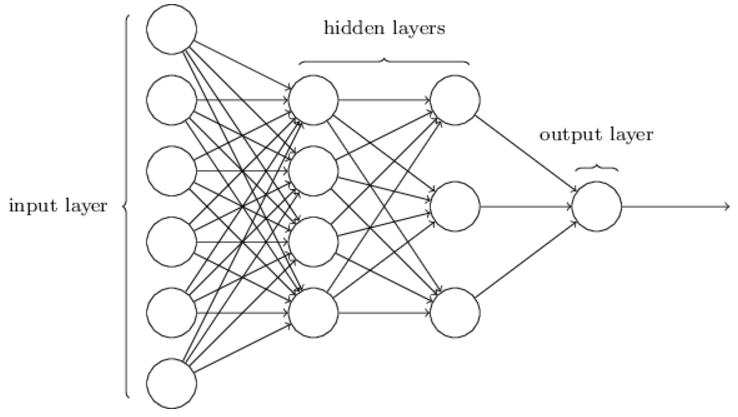
\includegraphics[scale=0.6]{Bilder/neural_network_extended}
	\caption{Aufbau des neuronalen Netzwerks hinsichtlich der einzelnen Layer.} 
	\label{fig:neural_network_extended} 
\end{figure}

\noindent
Für die Zusammensetzung von Eingabe- und Ausgabeschichten in einem Netzwerk, fällt die Betrachtung auf die Erkennung einer handgeschrieben "9". Als Eingabewerte dienen dem Netzwerk die Intensitäten der Bildpixel. Liegt ein Graustufenbild der Größe von 64x64 Pixeln vor, leiten sich daraus 4096 Eingabeknoten  mit skalierten Intensitätswerten zwischen 0 und 1 ab. Die Ausgabeschicht beinhaltet dagegen nur ein Neuron, um eine entsprechende Klassifizierung der "9" vornehmen zu können. \\[0.2cm]
\hspace*{1.3cm}
$ 
\begin{array}[t]{lcll}
	\mathtt{output} < 0.5 \quad\rightarrow\quad \mbox{"Eingabebild ist keine 9"} \\[0.2cm]
	\mathtt{output} \geq 0.5 \quad\rightarrow\quad \mbox{"Eingabebild ist eine 9"}
\end{array}
$
\\[0.2cm]
Im Vergleich hierzu ist der Aufbau der Hidden-Layer nicht durch irgendwelche Regeln ableitbar. Zum Einsatz kommen Heuristiken, die das Verhalten eines Netzwerkes bestimmen, welches ausgehend vom Experiment erwartet und gewünscht wird. Zum Beispiel kann Untersucht werden, wie die Lernrate des Netzwerks sich im Verhältnis zu der Anzahl an Hidden-Layer verhält. \\

\noindent
Bisher viel die Betrachtung in dieser Arbeit auf neuronale Netze, bei denen die Ausgabe einer Schicht die Eingabe in der nächsten Schicht darstellte. Solche Netzwerke werden auch \textit{Feedforward Neural Networks} bezeichnet. Hierunter ist das das nicht Auftreten von Schleifen zu verstehen - sprich, Informationen werden im Netzwerk immer von Layer $n$ zu Layer $n+1$ übergeben. Somit kann verhindert werden, dass das Netzwerk in gewissen Fällen bei der Eingabe der Sigmoid-Funktion $\sigma$ von dessen Ausgabe abhängig ist. \\
Ebenfalls gibt es Netzwerke bei denen sogenannte \textit{Feedback Loops} möglich sind. In diesem Fall handelt es sich um \textit{Recurrent Neural Networks}. Die Idee hinter diesem Modell ist, dass bestimmte Neuronen über einen definierten Zeitraum aktiv sind bevor sie inaktiv werden. Dies kann andere Neuronen anregen, ebenfalls über einen gewissen Zeitraum aktiv zu sein und eine entsprechende Kettenreaktion auslösen (Kaskade). Schleifen stellen in diesem Modell kein Problem dar, da die Ausgabe eines Neurons erst zu einem späteren Zeitpunkt die Eingabe beeinflusst. \\
Stellt man diese Arten von neuronalen Netzwerken gegenüber, so lässt sie zum heutigen Zeitpunkt die Aussage treffen, dass Feedback Neural Networks weniger Verbreitung finden. Dies ist begründet in der Leistungsfähigkeit der Lernalgorithmen. Jedoch sollte an dieser Stelle berücksichtigt werden, dass mittels Feedback Neural Networks bestimmte Probleme mit einem geringeren architektonischen Aufwand gelöst werden können. Darüber hinaus bildet der komplexere logische Aufbau eines solchen Netzwerks, das menschliche Verhalten besser ab.

\section{Perceptrons}
Ein Perceptron ist ein mathematisches Modell zur Abbildung eines künstliches Neurons in einem Netzwerk. Es wird für die Entscheidungsfindung herangezogen, indem verschiedene Aussagen abgewägt werden. Hierbei nimmt das Perceptron eine Menge von Eingaben $x_n$ mit $n \in \{1, \cdots, m\}$ und berechnet einen einzigen binären Ausgabewert (siehe Abb. \ref{fig:perceptron}). 
\begin{figure}[hbt]
	\centering
	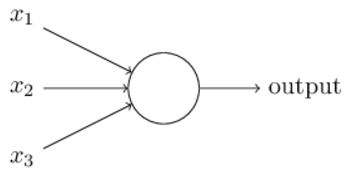
\includegraphics[scale=0.6]{Bilder/perceptron}
	\caption{Percetron mit den Eingaben $x_1, x_2, x_3$ und der Ausgabe $\mathtt{output}$.} 
	\label{fig:perceptron} 
\end{figure}

\noindent
Für jeden Eingabewert $x_n$ wird eine Gewichtung $w_n$ mit $n \in \{1, \cdots, m\}$ zugeordnet. Der Ausgabewerte $\mathtt{output}$ wird mittels der gewichteten Summe $\sum_j w_j x_k$ und einem definierten Grenzwert $\mathtt{threshold}$ bestimmt.
\begin{equation}
	\mathtt{output} := \left\{
	\begin{array}{ll}
 		0 & \displaystyle \mbox{falls}\quad \sum\limits_j w_j x_j \leq \mathtt{threshold} \\[0.5cm]
 		1 & \displaystyle \mbox{falls}\quad \sum\limits_j w_j x_j > \mathtt{threshold}
	\end{array}\right.
\end{equation}

\noindent
Der Aufbau des Netzwerks leitet sich aus den unterschiedlichen Modellen der Entscheidungsfindung ab und wird mit Hilfe der Perceptrons abgebildet (siehe Abb. \ref{fig:perceptron_models}).
\begin{figure}[hbt]
	\centering
	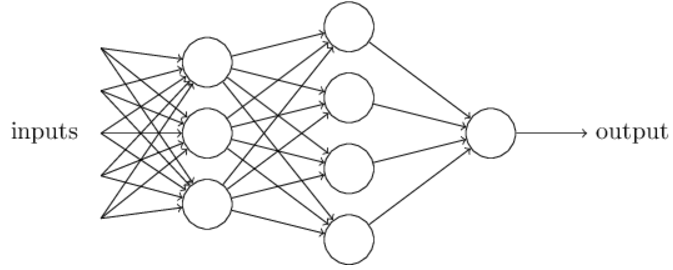
\includegraphics[scale=0.75]{Bilder/perceptron_models}
	\caption{Unterschiedliche Möglichkeiten der Entscheidungsfindung.} 
	\label{fig:perceptron_models} 
\end{figure}
Eine Entscheidungsmöglichkeit wird hierbei durch das Perceptron dargestellt. Weiterhin wird eine Spalte von Perceptrons als \textit{Layer} bezeichnet. Der erste Layer fällt Entscheidungen auf Basis der Eingabewerte, indem er diese abwägt. Jedes Perceptron des zweiten Layers hingegen, wägt für die Entscheidungsfindung die Resultate des ersten Layers ab. Ein Perceptron auf dem zweiten Layer kann somit eine Entscheidung auf einer abstrakteren und komplexeren Ebene durchführen. Auf diese Weise kann sich ein vielschichtiges Netzwerk von Perceptrons in ein anspruchsvolles Modell zur Entscheidungsfindung entwickeln. \\

\noindent
Im folgenden wird die mathematische Beschreibung von Perceptrons vereinfacht, indem Änderungen an der Notation für $\sum_j w_j x_j > \mathtt{threshold}$ vorgenommen werden. Für die Beschreibung der Summe $\sum_j w_j x_j$ werden die Vektoren $w$ und $x$ eingeführt, wodurch sich die Schreibweise $w \cdot x \equiv \sum_j w_j x_j$ ergibt. Des Weiteren wird der $\mathtt{threshold}$ auf die andere Seite der Ungleichung gezogen und erhält die Bezeichnung \textit{Bias}, $b \equiv \mathtt{-threshold}$. 
\begin{equation}
	\mathtt{output} := \left\{
	\begin{array}{ll}
 		0 & \displaystyle \mbox{falls}\quad w \cdot x + b \leq 0 \\[0.2cm]
 		1 & \displaystyle \mbox{falls}\quad w \cdot x + b > 0
	\end{array}\right.
\end{equation}
Somit nimmt der Bias Einfluss auf die binäre Ausgabe $\mathtt{output}$, weshalb der Bias eine Ausgabe mit einem hohen positiven oder negativen Wert mit einer höheren Wahrscheinlichkeit bedingen kann. \\

\noindent
Im vorherigen Abschnitt wurden Perceptrons als ein Methode für die Entscheidungsfindung beschrieben. Ein weiterer Anwendungsfall besteht in der Berechnung von logischen Funktion wie z.B. $\mathtt{AND}$, $\mathtt{OR}$ und $\mathtt{NAND}$. Fällt die Betrachtung auf ein Perceptron mit 2 Eingaben deren Gewichtung jeweils den Wert -2 aufweisen und einen Bias von 3, so ergibt sich folgende Abbildung (siehe Abb. \ref{fig:perceptron_example}).
\begin{figure}[hbt]
	\centering
	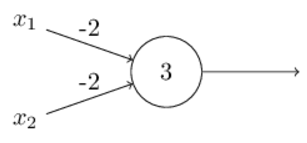
\includegraphics[scale=0.6]{Bilder/perceptron_example}
	\caption{Percetron mit zwei Eingaben -2 und einem Bias von 3.} 
	\label{fig:perceptron_example} 
\end{figure}

\noindent
Weisen die Eingaben $x_1, x_2$ den Wert 0 auf, ergibt sich für den $\mathtt{output}$ den Wert 1. Sind die Eingabewerte für $x_1, x_2$ -1 ergibt sich für den $\mathtt{output}$ den Wert -1. Der Aufbau beschreibt somit einen $\mathtt{NAND}$ Gatter.\\[0.2cm]
\hspace*{1.3cm}
$
\begin{array}[t]{lcll}
	w \cdot x + b & = & \mathtt{output} \\[0.2cm]
	(-2)*0+(-2)*0+3 & = & 1 \\[0.2cm]
	(-2)*1+(-2)*1+3 & = & -1
\end{array}
$
\\[0.2cm]
$\mathtt{NAND}$ Gatter können verwendet werden, um die unterschiedlichsten Berechnungen durchzuführen. Im Folgenden fällt die Betrachtung auf die Addition von zwei Bits $x_1$ und $x_2$. Für die Berechnung wird die bitweise Summe $x_1 \oplus x_2$ gebildet, wobei ein $\mathtt{carry bit}$ den Wert 1 annimmt, sobald $x_1$ und $x_2$ gleich 1.
\begin{figure}[hbt]
	\centering
	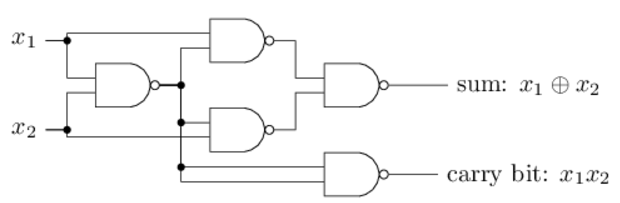
\includegraphics[scale=0.6]{Bilder/nand_gatter}
	\caption{$\mathtt{NAND}$ Gatter mit den Eingaben $x_1$ und $x_2$.} 
	\label{fig:nand_gatter} 
\end{figure}

\noindent
Um ein gleichwertiges Netzwerk abzuleiten, werden die $\mathtt{NAND}$ Gatter durch Perceptrons mit jeweils 2 Eingaben ersetzt. Hierbei weisen die Gewichtungen $w_1, w_2$ den Wert -2 und der Bias $b$ den Wert 3 auf. 
\begin{figure}[hbt]
	\centering
	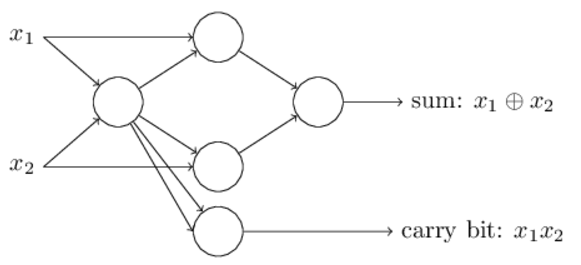
\includegraphics[scale=0.6]{Bilder/nand_gatter_perceptron}
	\caption{$\mathtt{NAND}$ Gatter Aufbau mit Perceptrons.} 
	\label{fig:nand_gatter_perceptron} 
\end{figure}

\noindent
In einem weiteren Schritt wird die Abbildung eines $\mathtt{NAND}$ Gatter mit Perceptrons vereinfacht. Dazu werden mehrere Eingänge eines Perceptrons zu einem zusammengefasst, weshalb aus den zwei Eingaben -2 der Wert -4 resultiert. Ebenfalls werden die Eingaben in einem sogenannten \textit{Input Layer} zusammengefasst, wobei durch die Notation eine Eingabe nicht mit einem Perceptron gleichzustellen ist.
\begin{figure}[hbt]
	\centering
	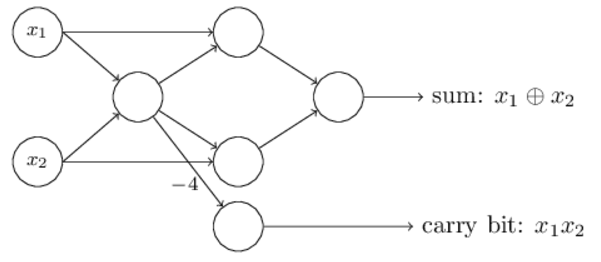
\includegraphics[scale=0.6]{Bilder/nand_gatter_perceptron_simplified}
	\caption{Vereinfachter $\mathtt{NAND}$ Gatter Aufbau mit Perceptrons.} 
	\label{fig:nand_gatter_perceptron_simplified} 
\end{figure}

\noindent
Dieser Anwendungsfall zeigt, dass mit Perceptrons unterschiedliche Berechnungen durchgeführt werden können. Implementierte Lernalgorithmen können Gewichtungen sowie den Bias automatisch durch entsprechende Stimuli im Netzwerk anpassen und ermöglichen die Nutzung von künstliche Neuronen, die sich von herkömmlichen Logik Gattern unterscheiden. Neuronale Netze können somit über einen definierten Zeitraum lernen, wie bestimmte Probleme zu lösen sind. 

\section{Sigmoid Neurons}
Für die Entwicklung lernender Algorithmen in einem Netzwerk mit Perceptrons, fällt unsere Betrachtung auf das Beispiel der Erkennung von handgeschriebenen Zahlen. Die Eingabe für das Netzwerk könnten die Raw Pixeldaten der eingescannten Bilder darstellen, welche die handgeschriebenen Zahlen abbilden. Das Ziel an dieser Stelle ist, dass das Netzwerk anhand der Veränderungen von \textit{Weights} und \textit{Biases} lernt eine korrekte Klassifizierung der Zahlen vorzunehmen. \\
Das Modifizieren der \textit{Weights} und \textit{Biases} kann das Verhalten des Netzwerkes und deren Entscheidungsfindung zu Problemen beeinflussen. Angenommen die Erkennung und Klassifizierung einer Zahl wurde durch das Netzwerk falsch vorgenommen, so können durch kleine Veränderungen an den \textit{Weights} und \textit{Biases} eine Korrektur durchgeführt werden. Dieses stetige Modifizieren der Werte über einen definierten Zeitraum ermöglicht ein lernendes Netzwerk (siehe Abb. \ref{fig:sigmoid_learning}). 
\begin{figure}[hbt]
	\centering
	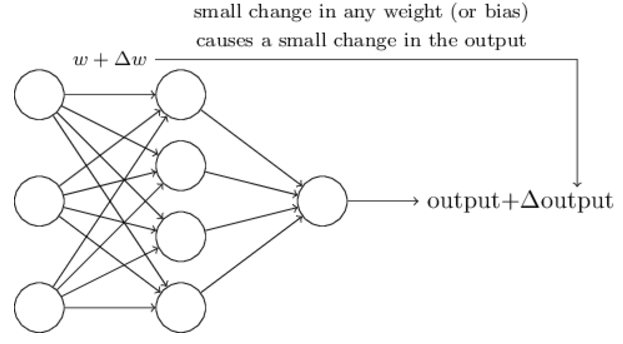
\includegraphics[scale=0.7]{Bilder/sigmoid_learning}
	\caption{Modifizieren von Weights und Biases schaffen lernendes Netzwerk.} 
	\label{fig:sigmoid_learning} 
\end{figure}

\noindent
Dieses wünschenswerte Verhalten eines lernenden Netzwerks kann durch Perceptrons nicht gewährleistet werden, da eine Veränderung der Weights und Biases den Ausgabewerte $\mathtt{output}$ eines Neurons umkehren kann. Dadurch kann das komplette Verhalten zur Klassifizierung von Zahlen beeinflusst werden, wobei zuvor falsch erkannte Zahlen nun richtig klassifiziert werden und umgekehrt. Mit Hilfe der Einführung des Sigmoid Neurons soll dieser Fehler behoben werden. Eine Änderung der Weights und Biases bei diesem künstlichen Neuron soll nur marginale Änderungen an dem Ausgabewert $\mathtt{output}$ vornehmen. Diese Erweiterung des Neurons begünstigt ein Netzwerk selbständig die Klassifizierung von Zahlen zu optimieren. \\

\noindent
Der Aufbau des Sigmoid Neurons ähnelt dem Perceptron, wobei das Neuron eine Anzahl von Eingabewerten $x_n$ mit $n \in \{1, \cdots ,m\}$ entgegennimmt und ausgehend von diesen Informationen den $\mathtt{output}$ ermittelt. Der wesentliche Unterschied zwischen diesen zwei Typen von Neuronen liegt in dem Wertebereich des $\mathtt{output}$. Bei dem Sigmoid Neuron kann dieser alle Werte zwischen 0 und 1 annehmen, sprich $\mathtt{output} \in [0 .. 1]$. Weiterhin weist auch diese Art von Neuronen für jeden Eingabewert eine Gewichtung $w_n$ mit $n \in \{1 .. n\}$ sowie einen Bias auf. \\
Für die Berechnung des $\mathtt{output}$ wird in diesem Kontext die \textit{Sigmoid Funktion} $\sigma(z)$ angewendet.
\begin{equation}
	\sigma(z) \equiv \frac{1}{1+e^{-z}} \quad\mbox{mit}\quad z = w \cdot x + b
\end{equation}
Unter Berücksichtigung der Eingabewerte $x_n$ mit $n \in \{1 .. n\}$ und der Weights  $w_n$ mit $n \in \{1 .. n\}$ ergibt sich die folgende Formel:
\begin{equation}
	\sigma(z) \equiv \frac{1}{1+\exp(-\sum_j w_j x_j - b)}
\end{equation}
Dabei weist das Sigmoid Neuron weiterhin das gleiche Verhalten wie ein Perceptron auf, wenn eine Grenzwertbetrachtung durchführt wird. \\[0.2cm]
\hspace*{1.3cm}
$
\begin{array}[t]{lcll}
	\lim\limits_{z \to \infty}{\sigma(z)} \approx 1 \quad\quad bzw. \\[0.2cm]
	\lim\limits_{z \to -\infty}{ \sigma(z)} \approx 0
\end{array}
$
\\[0.2cm]
Dieses Verhalten wird weiterhin verdeutlicht, wenn die Betrachtung auf den folgenden Funktionsgraph fällt (siehe Abb. \ref{fig:sigmoid_plot}). Für große $z$ nimmt die Funktion den Wert 1 an und für kleine $z$ nimmt die Funktion den Wert 0 an.
\begin{figure}[hbt]
	\centering
	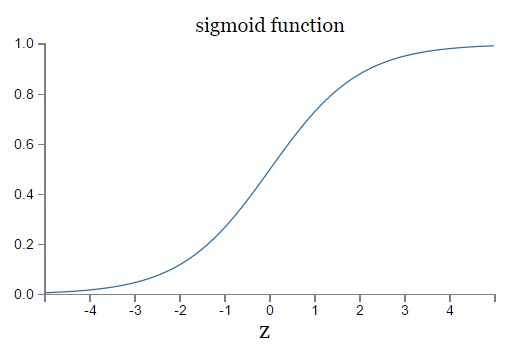
\includegraphics[scale=0.6]{Bilder/sigmoid_plot}
	\caption{Sigmoid Funktion $\sigma(z)$.} 
	\label{fig:sigmoid_plot} 
\end{figure}

\noindent
Im Vergleich hierzu die Stufenfunktion, die das Verhalten eines Perceptrons abbildet (siehe Abb. \ref{fig:perceptron_plot}).
\begin{figure}[hbt]
	\centering
	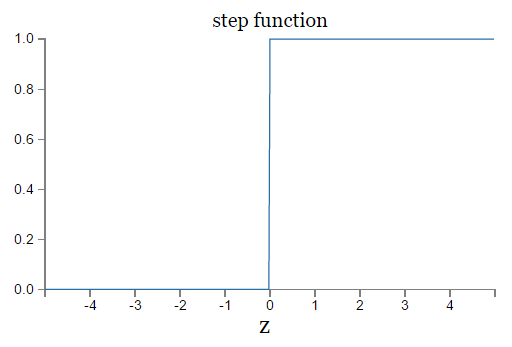
\includegraphics[scale=0.6]{Bilder/perceptron_plot}
	\caption{Sigmoid Funktion $\sigma(z)$.} 
	\label{fig:perceptron_plot} 
\end{figure}
Die Vorteile der Sigmoid Funktion liegen in den marginalen Änderungen $\delta w_j$ bei den Gewichtungen und $\delta b$ im Bias, welche eine marginale Änderung am $\delta\mathtt{output}$ vornehmen. Damit stellt $\delta\mathtt{output}$ die lineare Funktion bezüglich der Änderungen  $\delta w_j$ und $\delta b$ in den Weights und Bias dar.
\begin{equation}
	\Delta\mathtt{output} \equiv \sum_{j}{\frac{\partial\mathtt{output}}{\partial w_j}\Delta w_j+\frac{\partial\mathtt{output}}{\partial b}\Delta b_j}
\end{equation}
Diese Linearität begünstigt die Wahl von kleinen Änderungen in den Weights und Biases, um das Verhalten für ein lernendes Netzwerk abzuleiten.   

\section{Netzwerk zur Klassifizierung von handgeschrieben Zahlen}

%\bibliographystyle{alpha}
\bibliography{cs}
%\bibliography{/Users/stroetma/Dropbox/Kurse/cs}

\end{document}



